\section{Art Cohesion Test}
As the character art assets are being developed by multiple members of \ourteam{}, the differences between each artist's preferred art style may cause the art assets to be visually incompatible. In order to evaluate how effectively each artist's assets match the game's intended art style, surveys will be conducted with potential players. During these surveys, participants will be presented with 12 cards, each with a unique character printed onto them, designed by the four members of \ourteam{}'s art department. Each member designed three characters used in the test. The test subject will be told that between 1 and 6 artists created the group of characters, and that not every potential artist designed the same amount of characters. They will then be asked to group each character design by the artist(s) they believed made them, based on style. Once the test subject has sorted all of the cards, they will be asked to give their reasoning for their choices. Test subjects will then be asked if they believe that all the characters can exist in the same universe, and to record their thoughts using a Likert scale where 1 is Strongly Disagree, and 5 is Strongly Agree. They will then be asked to explain their reasoning for their ranking.

An example of the survey tools are shown in Figure~\ref{fig:survey}.

\begin{figure}[htb]
\centering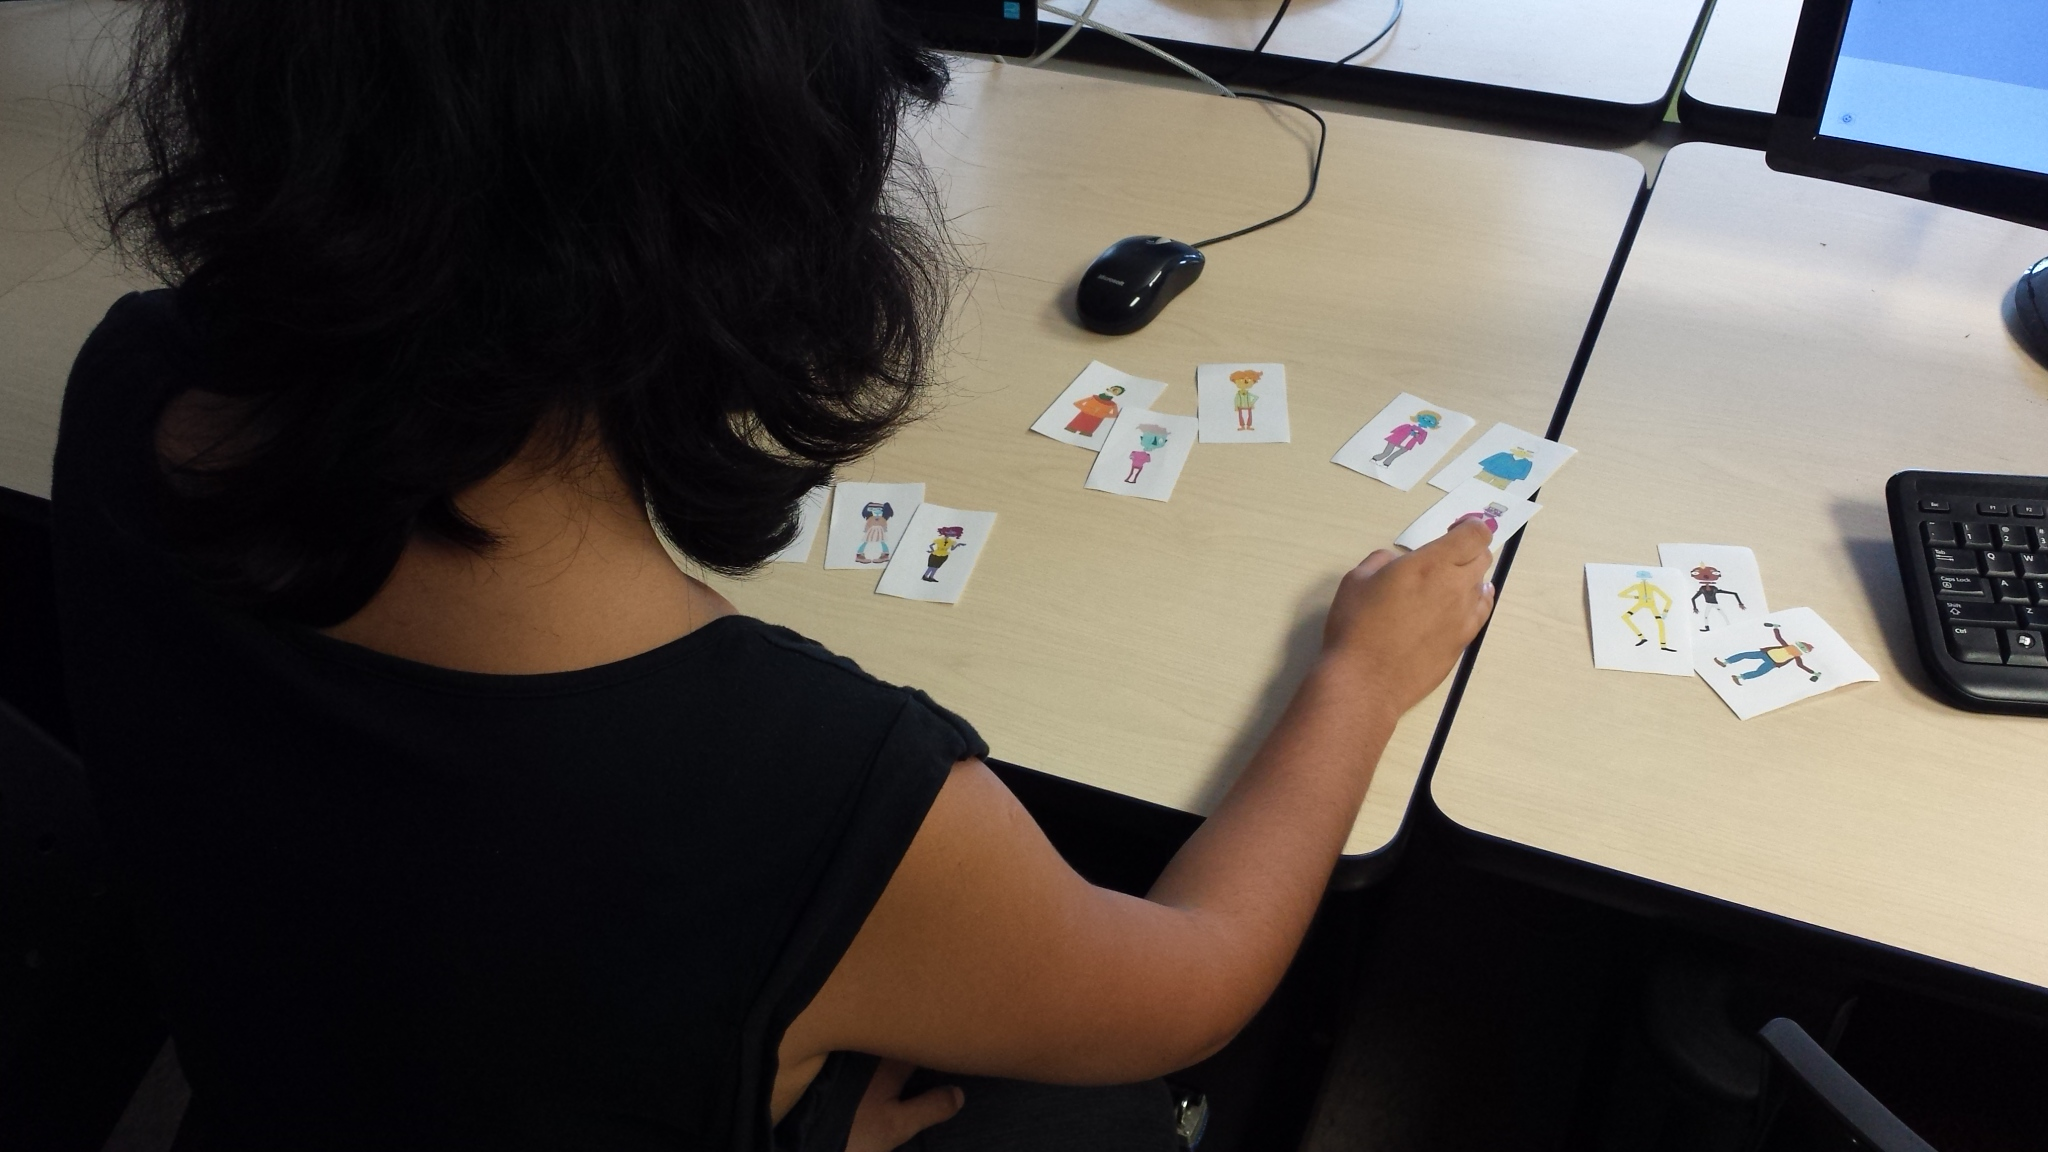
\includegraphics[width=.35\linewidth]{images/art_cohesion_test}
\caption{Artistic Cohesion Survey Tools}
\label{fig:survey}
\end{figure}

If participants are able to correctly place assets created by a single artist in the same group, and provide one or more logical reasons for their grouping, this may indicate that the artist has failed to match the intended vision. Together, the artists can evaluate the feedback and attempt to identify and ameliorate the visual elements that participants feel are jarring or out-of-place.